\documentclass [12pt,letterpaper]{article}
%Page margins, header and footer positions
\usepackage{geometry}
\usepackage[T1]{fontenc} % font encoding
\usepackage[utf8]{inputenc} 
\usepackage[italian,english]{babel}

%To display filling dots in the TOC for all entries
\usepackage[titles]{tocloft}
\renewcommand{\cftsecleader}{\cftdotfill{\cftdotsep}}

%Define new header and footer style
\usepackage{fancyhdr}

%graphics
\usepackage{graphicx}
\usepackage[dvipsnames, table]{xcolor}

%tables
\usepackage{tabu}
\usepackage{tabularx}
\usepackage{ltablex}
\usepackage{longtable}
\usepackage{float} % To allow the use of H modifier in long tables
\usepackage{multirow}

%url write style
\usepackage{xurl}

%bibliography
\usepackage{csquotes}
\usepackage[backend=biber, sorting=none, citestyle=numeric]{biblatex}
\addbibresource{bibliography.bib}
\usepackage{amsfonts}
\usepackage{amsmath}
\DeclareMathOperator{\argmax}{arg\,max}
\begin{document}
	%Title page
	\begin{titlepage}
        \title{Data Intelligence Applications\\Pricing and Matching}
		\date{2020/2021}
        \author{Ivan Cavadini (941927),\\Simone Marforio (944320),\\Nicolò Molinari (942404)}
		\maketitle
		\begin{center}
			
\includegraphics[scale=0.5]{Images/PolimiLogo}
		\end{center}
\end{titlepage}
	%Table of contents
	\tableofcontents
	%----
    \clearpage
    %---
	\section*{Introduction}
    \label{sect:Introduction}
    \addcontentsline{toc}{section}{Introduction}
	\subsection*{Scenario}
 Consider the scenario in which a shop has a number of promo codes to incentivize the customers that buy an item to buy a different item. The customers can belong to different classes and the promo codes can provide different discounts. 
\subsection*{Environment}
 Imagine two items (referred to as first and second items; for each item we have an infinite number of units) and four customers’ classes. The daily number of customers of each class is described by a potentially different (truncated) Gaussian probability distribution. Each class is also associated with a potentially different conversion rate returning the probability that the user will buy the first item at a given price.
\paragraph{}
Once a buyer has bought the item, she/he can decide to buy the second item that can be or not promoted. There are four different promos P0, P1, P2, P3, each corresponding to a different level of discount. P0 corresponds to no discount. Given the total number of customers, the business unit of the shop decides the number of promos as a fraction of the total number of the daily customers and is fixed (use two different settings in your experiments that you are free to choose). Each customers’ class is also associated with a potentially different conversion rate returning the probability that the user will buy the second item at a given price after she/he has bought the first. The promos will affect the conversion rate as they actually reduce the price. 
Every price available is associated with a margin obtained by the sale that is known beforehand. This holds both for the first and the second item. 
The conversion rates will change during time according to some phases due to, e.g., seasonality.
\subsection*{Steps}
\begin{enumerate}
\item Provide a mathematical formulation of the problem in the case in which the daily optimization is performed using the average number of customers per class. Provide an algorithm to find the optimal solution in the offline case in which all the parameters are known. Then, during the day when customers arrive, the shop uses a randomized approach to assure that a fraction of the customers of a given class gets a specified promo according to the optimal solution. For instance, at the optimal solution, a specific fraction of the customers of the first class gets P0, another fraction P1, and so on. These fractions will be used as probabilities during the day.
\item Consider the online learning version of the above optimization problem, identify the random variables, and choose a model for them when each round corresponds to a single day. Consider a time horizon of one year.
\item Consider the case in which the assignment of promos is fixed and the price of the second item is fixed and the goal is to learn the optimal price of the first item. Assume that the number of users per class is known as well as the conversion rate associated with the second item. Also assume that the prices are the same for all: the classes (assume the same in the following) and that the conversion rates do not change unless specified differently below. Adopt both an upper-confidence bound approach and a Thompson-sampling approach and compare their performance.
\item Do the same as Step 3 when instead the conversion rate associated with the second item is not known. Also assume that the number of customers per class is not known.
\item Consider the case in which prices are fixed, but the assignment of promos to users need to be optimized by using an assignment algorithm. All the parameters need to be learnt. 
\item Consider the general case in which the shop needs to optimize the prices and the assignment of promos to the customers in the case all the parameters need to be learnt.
\item Do the same as Step 6 when the conversion rates are not stationary. Adopt a sliding-window approach.
\item Do the same as Step 6 when the conversion rates are not stationary. Adopt a change-detection test approach.
\end{enumerate}
\subsection*{Context Modeling}
We have considered a ski shop that sells racing skis as first item and racing ski helmets as second item. The optimization problem have a time horizon of one year, splitted in three seasons that change the conversion rates of the two items. Customers are splitted into four different categories that define their purchasing behavior (conversion rates), according to the season and the price of the item.

\begin{center}
	\begin{tabular}{ |c|c|p{9cm}| } 
	\hline
	\multirow{3}{4em}{Items} & Racing Skis & Professional racing skis \\ 
	& Racing Ski Helmet &  Professional racing skis helmet\\ 
	\hline
	\multirow{3}{4em}{Customer categories} & Sport addicted & Who loves and practices ski frequently\\ 
	& Gifter &  Who wants to give away the both items\\
	& Worried &  Who pays a lot of attention to the price of the items\\ 
	& Amateur &  Who sometimes practices ski\\ 
	\hline
	\multirow{3}{4em}{Seasons} & Spring-Summer & Buyers are not tempted to spend a lot, ski season is far away\\ 
	& Autumn & Buyers are willing to spend in anticipation of the arrival of the ski season \\
	& Winter &  Ski season has begun, those who have not yet bought the equipment have hurried to buy it so as not to waste the season\\  
	\hline
	\end{tabular}
	\end{center}

\subsection*{Assumption}
\begin{itemize}
		\item Seasonality is taken into accout only for the 7$^{th}$, 8$^{th}$ requests, while for all the other, the seasonality of the products is not considered and the conversion rates remain static. For this requests the default season is the first one, in our context called Spring.  
		\item In our mathematical formulation, for the total reward maximization problem, we consider the production cost of both the items equal to zero.
		\item For the first step the objective of promo assignment is to find the best values for the fractions of clients of the various classes that receice a specific promo code. In the next steps, instead, we use online learning algorithm to find the best combination for the assignment promo code - class.
	\end{itemize}	
    %--
    \section*{Formal Model}
    \label{sect:Formal Model}
    \addcontentsline{toc}{section}{Formal Model}
	\subsection*{Variables definition}
\begin{itemize}
\item $i$= user category 
\item $j$ = promotional discount: P$_0$ = 0\%, P$_1$ = 10\%, P$_2$ = 20\%, P$_3$ = 30\%
\item $p1$ = full price of the first item (\textit{Racing skis}) 
\item $p2$ = full price of second item (\textit{Racing ski helmet})
\item $p2_j$ = price of the \textit{Racing ski helmet} when applied the promo $j$
\item $c1$ = production cost of \textit{Racing skis} = 0
\item $c2$ = production cost of \textit{Racing ski helmet} = 0
\item $q1_i(p1)$ = conversion rate for user category $i$, for \textit{Racing skis} sold at the price $p1$
\item $q2_i(p2)$ = conversion rate for user category $i$, for \textit{Racing ski helmet} sold at price the $p2$
\item $s_{ji}(p2)$ = discounted price of \textit{Racing ski helmet}, for user category $i$, according to promo discount $j$
\item $d_{ij}$ = amount of promo $j$ distributed to user category $i$
\item $d_{max}$ = maximum number of promos to be to distributed (\#P$_1$ + \#P$_2$ + \#P$_3$)
\item $avgCustomer_i$ = average number of customers for category $i$
\end{itemize}


\subsection*{Formulation of elaborated variables}
\begin{itemize}
\item $p1*q1_i(p1)*avgCustomer_i$ = revenue for the sale of \textit{Racing skis} at price $p1$ to user category $i$ 
\item $s_{ji}(p2)*q2_i(s_{ji}(p2))*d_{ij}*avgCustomer_i$  = revenue for the sale of \textit{Racing ski helmet} at the discounted price $p2$, according to the user-promo assignement 
\item $(p1*q1_i(p1)-c1*q1_i(p1))*avgCustomer_i$ = revenue for the sale of \textit{Racing skis} taking into account the production cost $c1$
\item $(q2_i(p2)*(s_{ji}(p2)*q2_i(s_{ji}(p2))*d_{ij}-q2_i(s_{ji}(p2)))*c2)*avgCustomer_i$ = revenue for the sale of \textit{Racing ski helmet} taking into account the production cost $c2$
\end{itemize}

\subsection*{Objective Function}
We have a maximization problem with the following objective function:\\
\\
$\textrm {max} ( \sum \limits _{i = 0, j = 0} ^{i = 4, j = 4}[(p1*q1_i(p1) - c1*q1_i(p1) + q2_i(p2)(s_{ji}(p2)*q2_i(s_{ji}(p2))*d_{ij} -  q2_i(s_{ji}(p2))*c2))*avgCustomer_i])$

\textbf{s.t:} $ \forall j>0 : [\sum \limits _{i = 0} ^{i = 4} d_{ij}] = d_{max} $
\\
We have fixed the full prices of the two items: $p1$, $p2$. We retrieve the discounted prices of $p2$, applying the promos $j$. \\
We know: the average number of customers per category $i$, $avgCustomer_i$, the conversion rate for both products ($q1_i(p1)$, $q2_i(p2)$) and the maximum number of promos to distribute ($d_{max}$).\\
As assumption the production costs of the two items is zero ($c1$ = 0, $c2$ = 0).\\
It is possible to retrieve the total revenue for \textit{Racing skis} as the product between the full price of the first item, the conversion rate for the considered user category and the average number of customers for that category:
$(p1 * q1_i(p1) * avgCustomer_i)$.\\
For the second item the calculation of the reward is the same except for the fact that the product is buyed only if also the first one is purchased (so we multiply also the conversion rate of the first item) and the considered price have to be discounted according to the assigned promotion. 

The solution of our optimization problem consists in the distribution of the fraction of promo codes among the user categories.

\subsection*{Offline problem - designed algorithm}

In this scenario we have to find the optimal solution in an offline manner (a solution to our maximization problem knowing all the parameters), considering the constraints that the shop uses a randomized approach to assure that a fraction of the customers of a given category gets a specified promotion according to the optimal solution.\\
We achieve the solution of the problem using a matching approach. 
To reach the optimal solution we have used an iterative approach: we build a matrix category-promotion containing the mean expected rewards for every couple, calculated as the conversion rate of the \textit{Racing ski helmet} multiplied with its discounted price.
The goal is to obtain, for each category-promotion couple the fraction of customers that will receive this discount.\\
We exploit this matrix to perform the matching between the customer classes and the promo types, in order to maximize the total reward. \\
We select the best reward for every class, for four times, retrieving, at every iteration, the four best combination of category-promotion and assigning an infinite weight to the obtained sub-optimal matching.\\
Every matching is represented by a reward configuration that maximize the total reward. Every iteration is weighted and represent a different goodnesses of the solution, the first is the best, the last is the worst.\\
Through the sub-optimal matchings, we have retrieved the fractions of different promos to assign to every customer categories, based on the proportional weight of the previous sub-optimal matching.\\
The proportions retrieved, are normalized category per category.

PESEUDOCODICE
\begin{center}
	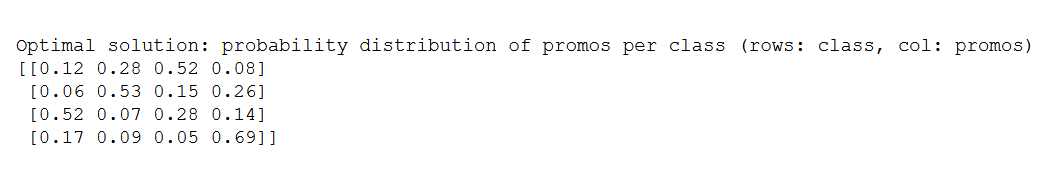
\includegraphics[scale=0.9]{Images/n1_results}
\end{center}
\begin{center}
	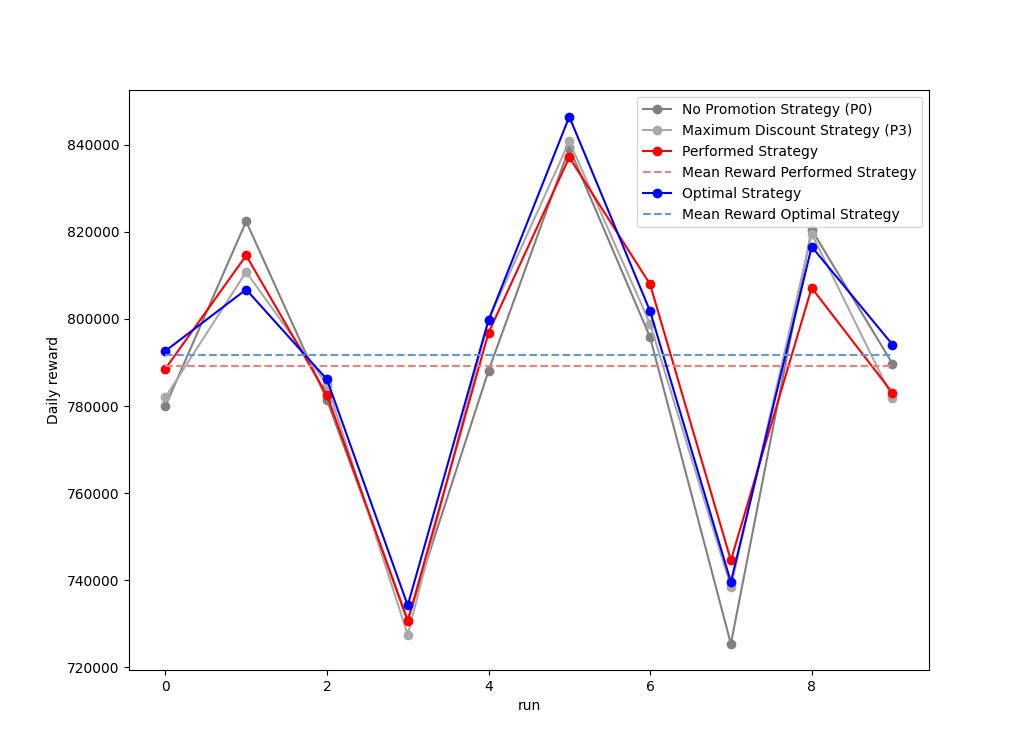
\includegraphics[scale=0.7]{Images/n1_chart}
\end{center}





	
    %---
    \section*{Random Variables}
    \label{sect:Random Variables}
    \addcontentsline{toc}{section}{Random Varaibles}
	Daily customers: Gaussian Distribution\\
Normalized gaussian parameters per class (normalizing factor:1000), average and variance:

\begin{tabularx}{0.8\textwidth} { 
		| >{\raggedright\arraybackslash}X 
		| >{\centering\arraybackslash}X 
		| >{\raggedleft\arraybackslash}X | }
	\hline
	Customer Category & Average & Variance  \\
	\hline
	Category 1 & 0.15 & 0.03  \\
	\hline
	Category 2 & 0.20 & 0.03  \\
	\hline
	Category 3 & 0.40 & 0.05  \\
	\hline
	Category 4 & 0.25 & 0.04  \\
	\hline
\end{tabularx}

\begin{center}
	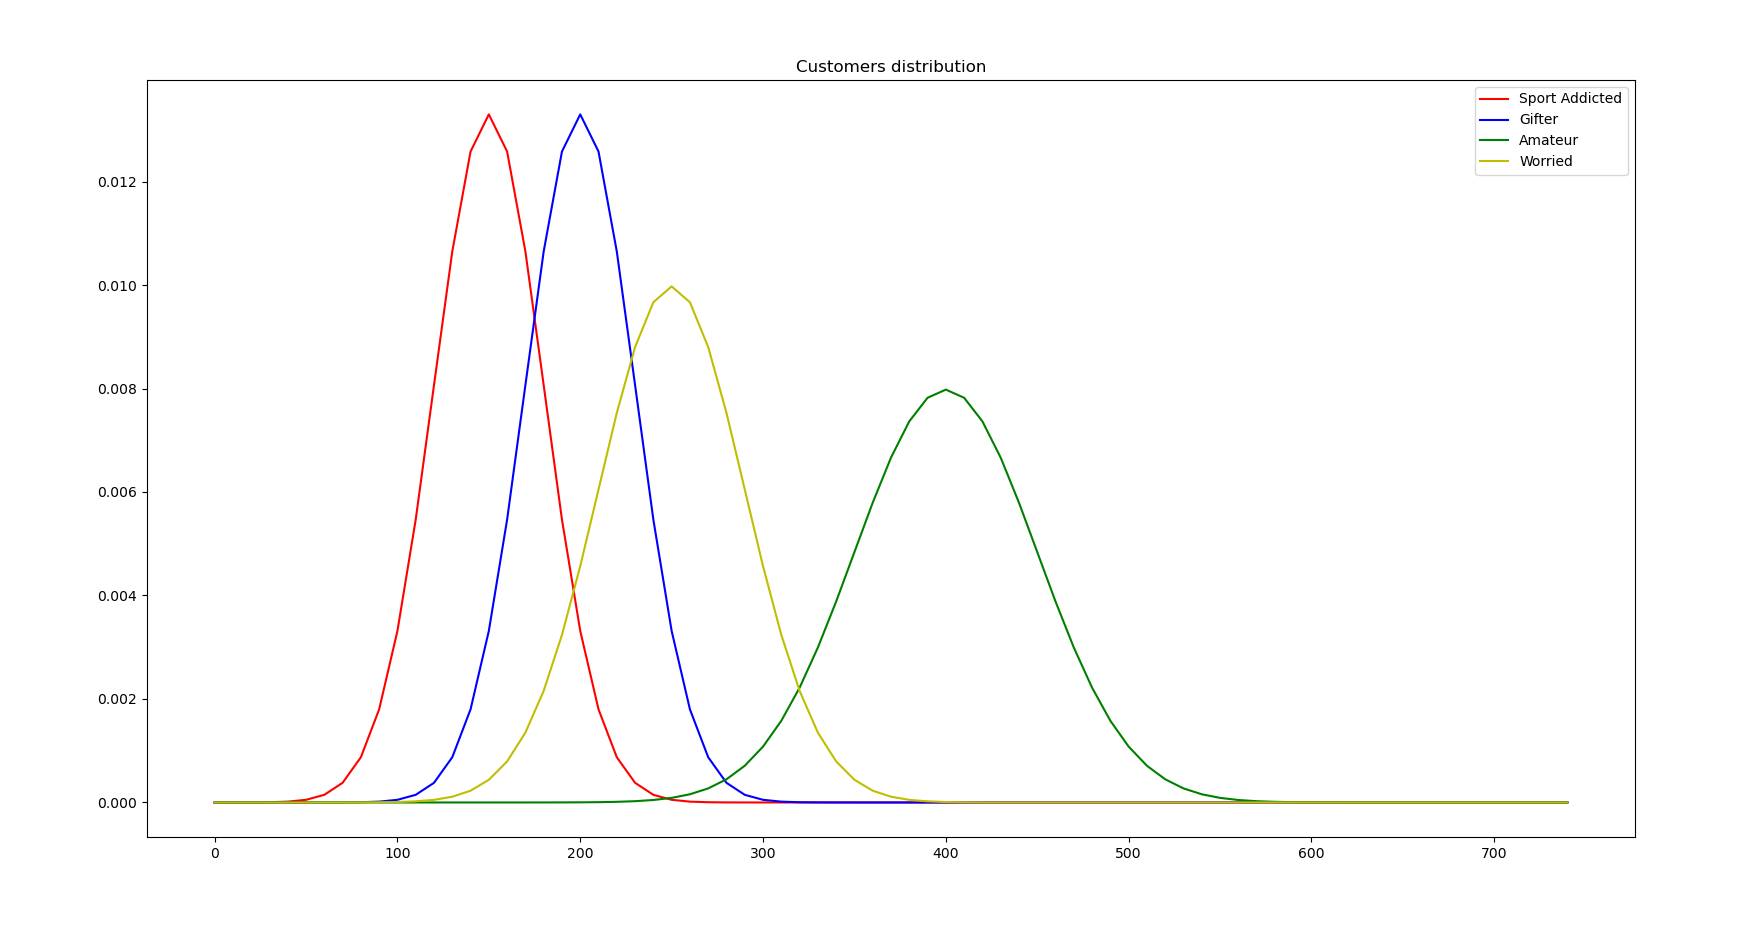
\includegraphics[scale=1]{Images/CustomerDistribution}
\end{center}


\begin{itemize}
	\item Buy item1(price) : Bernoulli \~ 0,1
	\item Buy item2(price) : Bernoulli \~ 0,1
	\item Reward item1 = buy item 1 * price item 1
	\item Reward item2 = buy item 1 * buy item 2 * price item2
	\item Time horizon = 365 days
\end{itemize}
The following graphs are the demand curves of the two item: the first three graphs are the demand curves of the first item, associated to the three seasonality (spring-summer, autumn, winter); the last three graphs are the demand curves of the second item with its respective seasonality.
\begin{center}
	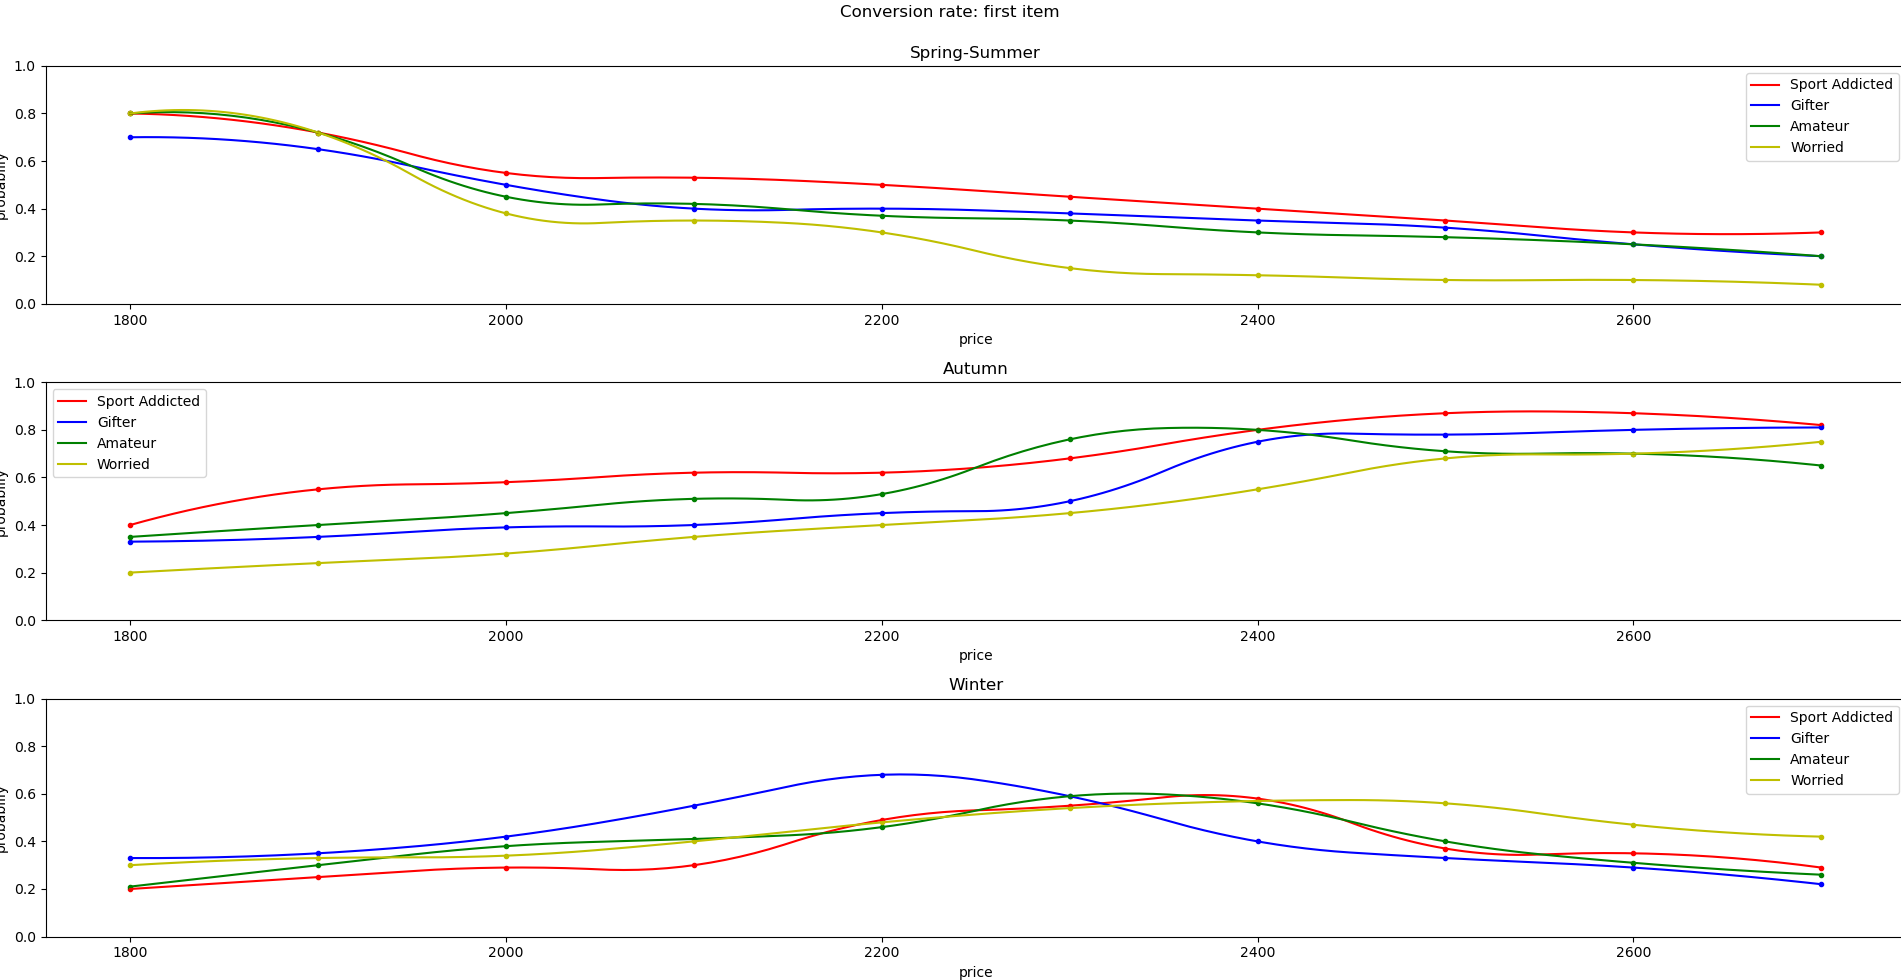
\includegraphics[scale=0.5]{Images/CR_fstItem}
\end{center}

\begin{center}
	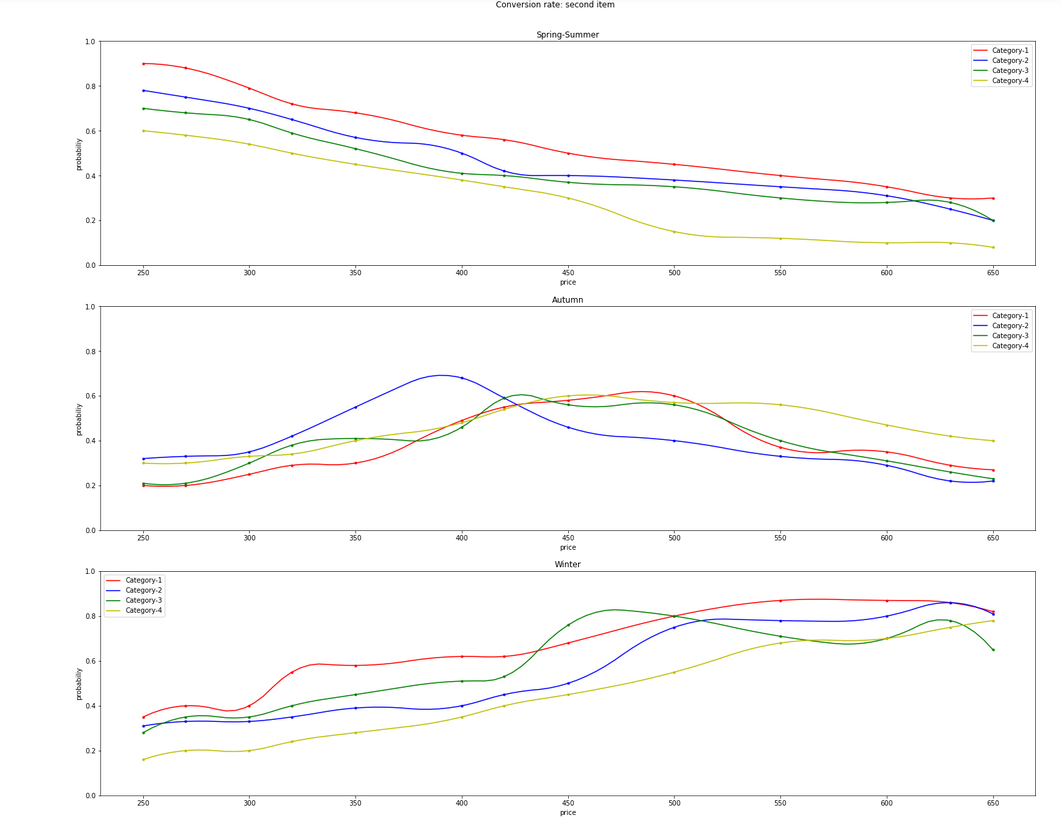
\includegraphics[scale=0.5]{Images/CR_scndItem}
\end{center}

\subsection{Online Approach}
Daily we extract the items prices using an online learner algorithm (pricing or matching), then we simulate the current day estimating the number of customers per class through the gaussian distribution. The arrival of every customer is simulated with a random approach. The system proposes the first item to every customer, simulating the purchase of it exploiting the associated Bernoulli distribution probability. The second item is proposed to the customer with the same approach, only if the first item will be bought. It is possible to exploit the information obtained in the previous steps to calculate the rewards and use them to update the learner. This procedure is repeated for every daily customer, for a time horizon of 365 days and during this period the purpose is to find a solution (composed by the prices and the assignment of promotions) that maximise the total reward. 		
    %---
    \section*{Online pricing for first item}
    \label{sect:Online pricing for first item}
    \addcontentsline{toc}{section}{Online pricing for first item}
	\subparagraph*{Submission : }
\textit{Consider the case in which the assignment of promos is fixed and the price of the second itm is fixed and the goal is to learn the optimal price of the first item. Assume that the number of users per class is known as well as the conversion rate associated with the second item. Also assume that the prices are the same for all: the classes (assume the same in the following) and that the conversion rates do not change unless specified differently below. Adopt both an upper-confidence bound approach and a Thompson-sampling approach and compare their performance.}\\

The request is to learn the optimal price of the first item, comparing the adoption of a Thompson-sampling approach and an Upper-Confidence Bound approach

\subsection*{Basic knowledge}
The described problem is a combinatorial bandit problem, which is a decision making problem in where decision maker selects one single arm in each round, and observes a realization of the corresponding unknown reward distribution. Each decision is based on past observed rewards. The objective is to maximize the expected cumulative reward over some time horizon by balancing exploitation and exploration. We can solve it, through an online algorithm, where only for the feasible solutions we will have precise estimations. Thomspon-Sampling algorithm (TS) and Upper-Confidence Bound algorithm (UCB1) are well known algorithm used to solve combinatorial bandits problem.

\subparagraph*{Upper-Confidence Bound (UCB1)}

\begin{itemize}
	\item Every arm is associated with an upper confidence bound 
	\item At every round, the arm with the highest upper confidence bound is chosen
	\item After having observed the realization of the reward of the arm, the upper confidence bound is updated
\end{itemize}
Notation:\\
\begin{itemize}
\item $t$ time
\item $A$ set of arms
\item $a$ arm
\item $a_{t}$ arm played at time $t$
\item $a^*$ optimal arm
\item $X_{a}$ random variable (bernoulli) associated to arm a
\item $\mu_{a}$ expected value of random variable $X_{a}$
\item $x_{a,t}$ realization of random variable $X_{a}$ at time $t$
\item $x_{a}$ realizations of $X_{a}$
\item $\bar{x}_{a}$ empirical mean of $x_{a}$
\item $n_{a}(t)$ number of samples of arm $a$ at time $t$
\end{itemize}

Pseudocode\\

1. Play once each arm $a \in A$

2. At every time $t$ play arm $a$ such that:

\hspace{2em}$a_{t} \leftarrow \argmax_a{\left\{\left[\bar{x}_{a} + \sqrt{\frac{2 log(t)}{{n_{a}(t-1)}} }\right]\times a\right\}}$

\subparagraph*{Thompson Sampling (TS)}

\begin{itemize}
	\item For every arm, we have a prior on its expected value 
	\item In the case the arms’ rewards are Bernoulli distribution, the priors are Beta distributions
	\item Notice that, with the opportune parameters, a Beta distribution is a uniform distribution 
	\item For every arm, we draw a sample according to the corresponding Beta
	\item We choose the arm with the best sample 
	\item We update the Beta distribution of the chosen arm according the observed realization
\end{itemize}

Notation (in addition to classical UCB):\\
\begin{itemize}
	\item $\mathbb P(\mu_{a}=\theta_{a})$ prior of the expected value of $X_{a}$
	\item $\theta_{a}$ variable of $\mathbb P(\mu_{a}=\theta_{a})$
	\item $(\alpha_{a_{t}}, \beta_{a_{t}})$ parameters of the beta distribution $P(\mu_{a}=\theta_{a})$
\end{itemize}

Pseudocode\\

1. At every time $t$ for every arm $a$:

\hspace{2em}$\tilde{\theta_{a}} \leftarrow Sample(\mathbb P(\mu_{a}=\theta_{a}))$ \\

2. At every time $t$ play arm $a_{t}$ such that 

\hspace{2em}$a_{t} \leftarrow \argmax_a \left\{ \tilde{\theta_{a}} \times a \right\} $ \\

3.  Update beta distribution of arm $a_{t}$

\hspace{2em}$(\alpha_{a_{t}}, \beta_{a_{t}}) \leftarrow (\alpha_{a_{t}}, \beta_{a_{t}}) + (x_{a_{t},t}, 1 - x_{a_{t},t})$


\subsection*{Strategy}

In our solution we simulate a random arrival of the customers, through two different leaners, TS learner and a UCB learner, we extract from our candidates two prices and we emulate the purchase phase using both prices. In case the customer buys the first item, we propose the second one at a fixed price, computed according to the customer category. In this case we do not simulate the purchase phase, but we use the knowledge of the conversion rate of the second item to compute the final customer reward. 

\subparagraph{Implementation} 
\begin{itemize}
	\item No seasonality, conversion rate do no change
	\item Number of customers per class is known 
	\item Candidates for the \textit{Racing Skis} are: \{2260.0,1910.0,2130.0, 2010.0, 2340.0\}
	\item Conversion rate associated with the first item is not known
	\item Basic price of the Racing Ski Helmet is fixed to 630.0
	\item Promotion assignment is fixed, according to the results of our offline solution: 
	\begin{center}
		\begin{tabular}{ |c|c|c|} 
		\hline
		User category & Assigned promotion & Racing Ski Helmet price \\
		\hline
		Sport Addicted & P$_2$ : 20\% & 504.0 \\
		\hline
		Gifter & P$_1$ : 10\% & 567.0 \\
		\hline
		Amateur & P$_0$ : 0\% & 630.0 \\
		\hline
		Worried & P$_3$ : 30\% & 441.0 \\
		\hline
		\end{tabular}
	\end{center}
	\item Conversion rate associated with the second item is known
\end{itemize}

Both UCB and TS learner expect as learnign parameter a binomial value, while our reward is value composed by the sold of the first item plus the eventual sold of the second item. In order to normilize the reward to be passed learner, we divide the customer reward by the maximum achievable reward.   

\subparagraph{Optimal strategy}In order to compute a regret, the simulated rewards are compared with an optimal solution that, accordingly to the conversion rates for the first items, is to offer the \textit{Racing Skis} at the lower price (1910.0 according to our candidates prices). 

\subsection*{Results}
\begin{center}
	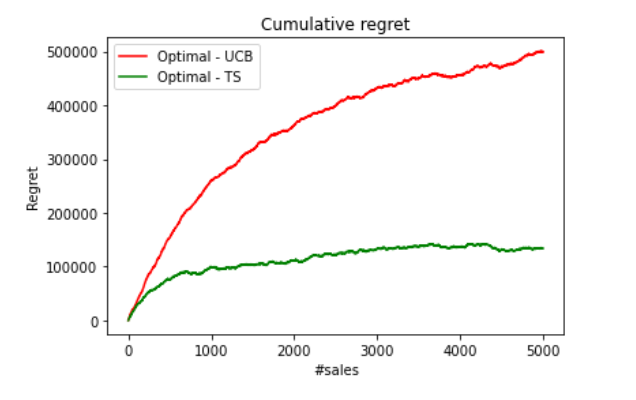
\includegraphics[scale=1.2]{Images/n3}
\end{center}
Days: 10\\
Experiments number: 10 \\
Both UCB and TS strategy converge on 1910.0\\
\textit{We decide to plot the regret of the first 5000 clients, since plotting the results of the entire time horizon made the plot unreadable}


\subsection*{Considerations}
As we can observe in the plot, both approach converge to a stable solution, however Thompson Sampling approach performs better than a UCB approach. Infact Thompson Sampling is faster to find the best price for the first item than UCB and this allow to have a lower regret. 	
    %---
    \section*{Online pricing for first item with purchase simulation}
    \label{sect:Online pricing for first item with purchase simulation}
    \addcontentsline{toc}{section}{Online pricing for first item with purchase simulation}
	\subparagraph*{Problem explaination}
\subparagraph*{Strategy}
\subparagraph*{Results}
\subparagraph*{Considerations}	
    %---
    \section*{Matching problem: promo assignment}
    \label{sect:Matching problem: promo assignment}
    \addcontentsline{toc}{section}{Matching problem: promo assignment}
	\subparagraph*{Submission : }
\textit{Consider the case in which prices are fixed, but the assignment of promos to users need to be optimized by using an assignment algorithm. All the parameters need to be learnt.}\\

The submission requires to learn the assignment of the promotions to the diffferent customer category. This time we are dealing with a matching problem. 

\subsection*{Basic knowledge}
DIRE CHE BANDIT PROBLEM è e RIVEDERE SE QUELLI PRECEDENTI SONO GIUSTI. AGGIUNGERE UN PO' DI TEORIA

A Matching Problem can be modeled as a graph $G=(N,A)$, where $N$ is a set of node and $A$ is a set of arc. A matching $M$ is a subset of $A$ such that each node is connected to at most one node with at most one arc of $M$. The problem can be seen as a maximization problem where the objective is to determine the matching of maximum cardinality.\\

\subparagraph*{UCB Matching}
We can design a bandit algorithom that solve the mathing problem. A classical UCB approach is combined with a linear sum assignement algorithm, a well known algorithm that given a bipartite graph solve the matching problem. The learner will retrieve a the subset of arc that correspond to the optimal matching. 
At $t$, play a superarm $a_{t}$ such that:\\
$a_{t} \leftarrow \argmax\limits_{\textbf{a} \in M}{\left\{\sum\limits_{a \in \textbf{a}}\bar{x}_{a,t} + \sqrt{\frac{2 log(t)}{{n_{a}(t-1)}} }\right\}}$ \\
where $M$ is the set of matches.

\subparagraph*{Promo-Category UCB Matching}

We have slightly modifying the previously implemented UCB Matching. \\
We introduce two matrixes, with the same shape of the promotion-category graph, used for the maximization problem, representing the matching between a specific customer category and a specific promo. The first matrix represent the total collected rewards for that specific assignement, the second is used as support and contains the number of occurences that the assignement has been chosen (a customer of that category to which it was proposed the second item with that promo). 
Those matrix are updated by the reward obtained by the currently served customer and used to calculate the average reward of each possible assignment. The average value are used to feed the default UCB Matching learner in order to update the confidence bound.
An initialization phase is needed in order to explore and learn the average reward for all the possible configurations. For this reason we introduce a staring dalay in which we explore all possible configurations in an exaustive way and store the rewards. In this phase the learner do not compute the optimal solution for the matching problem, but retrieves a known matching that change at each iteration.
As for the other learners, the rewards are normalized dividing the actual reward by the maximum possible reward.

\subsection*{Strategy}

As always we simulate the randomly arrival of the customers and the purchase at a fixed price of the first item. In case the customer purchase the \textit{Racing Skis}, we ask to the learner (our custom UCB matching learner) to retrieve the optimas assignemnt promotions-category. According to the user category, and the pulled assignment promo-category, we compute the discounted price for the second item and we propose it to the customer. In important to note that the learner provides us a set of arms, but we use only the assignement that involve the category of the currently served user. The user reward is calculated as the sum of the reward obtained by the sold of the first item plus the eventually sold of the sencond. However, since our goal it to lorne the matching for the fromo-category of the second item, and the price of the \textit{Racing Skis} is fixed, we feed the matching learner with the reward obtained by the sold of the \textit{Racing Ski Helmet}. 

\subparagraph{Implementation} 
\begin{itemize}
	\item No seasonality, conversion rate do no change
	\item Price of the \textit{Racing Skis} is fixed to 1980.0
	\item Conversion rate associated with the first item is not known
	\item Basic price of the \textit{Racing Ski Helmet} is fixed to 630.0
	\item Conversion rate associated with the second item is not known
	\item Optimal promotion-category assignment need to be learnt
\end{itemize}

\subparagraph{Optimal strategy}The optimal strategy, used to compute the regret, is calculated in an offline manner, calculating for each possible promotion-category the expected reward, obtained multiplyng the conversion rate of the category with the discounted price. The obtained matrix of the expected rewards is then evaluated with a Linear Sum Assignement algorithm that maximize the total expected reward, retrieving the optimal assigment. The obtained optimal solution is:\\
\begin{center}
	\begin{tabular}{ |c|c|c|} 
	\hline
	User category & Assigned promotion & Racing Ski Helmet price \\
	\hline
	Sport Addicted & P$_2$ : 20\% & 504.0 \\
	\hline
	Gifter & P$_1$ : 10\% & 567.0 \\
	\hline
	Amateur & P$_0$ : 0\% & 630.0 \\
	\hline
	Worried & P$_3$ : 30\% & 441.0 \\
	\hline
	\end{tabular}
\end{center}

\subsection*{Results}
\begin{center}
	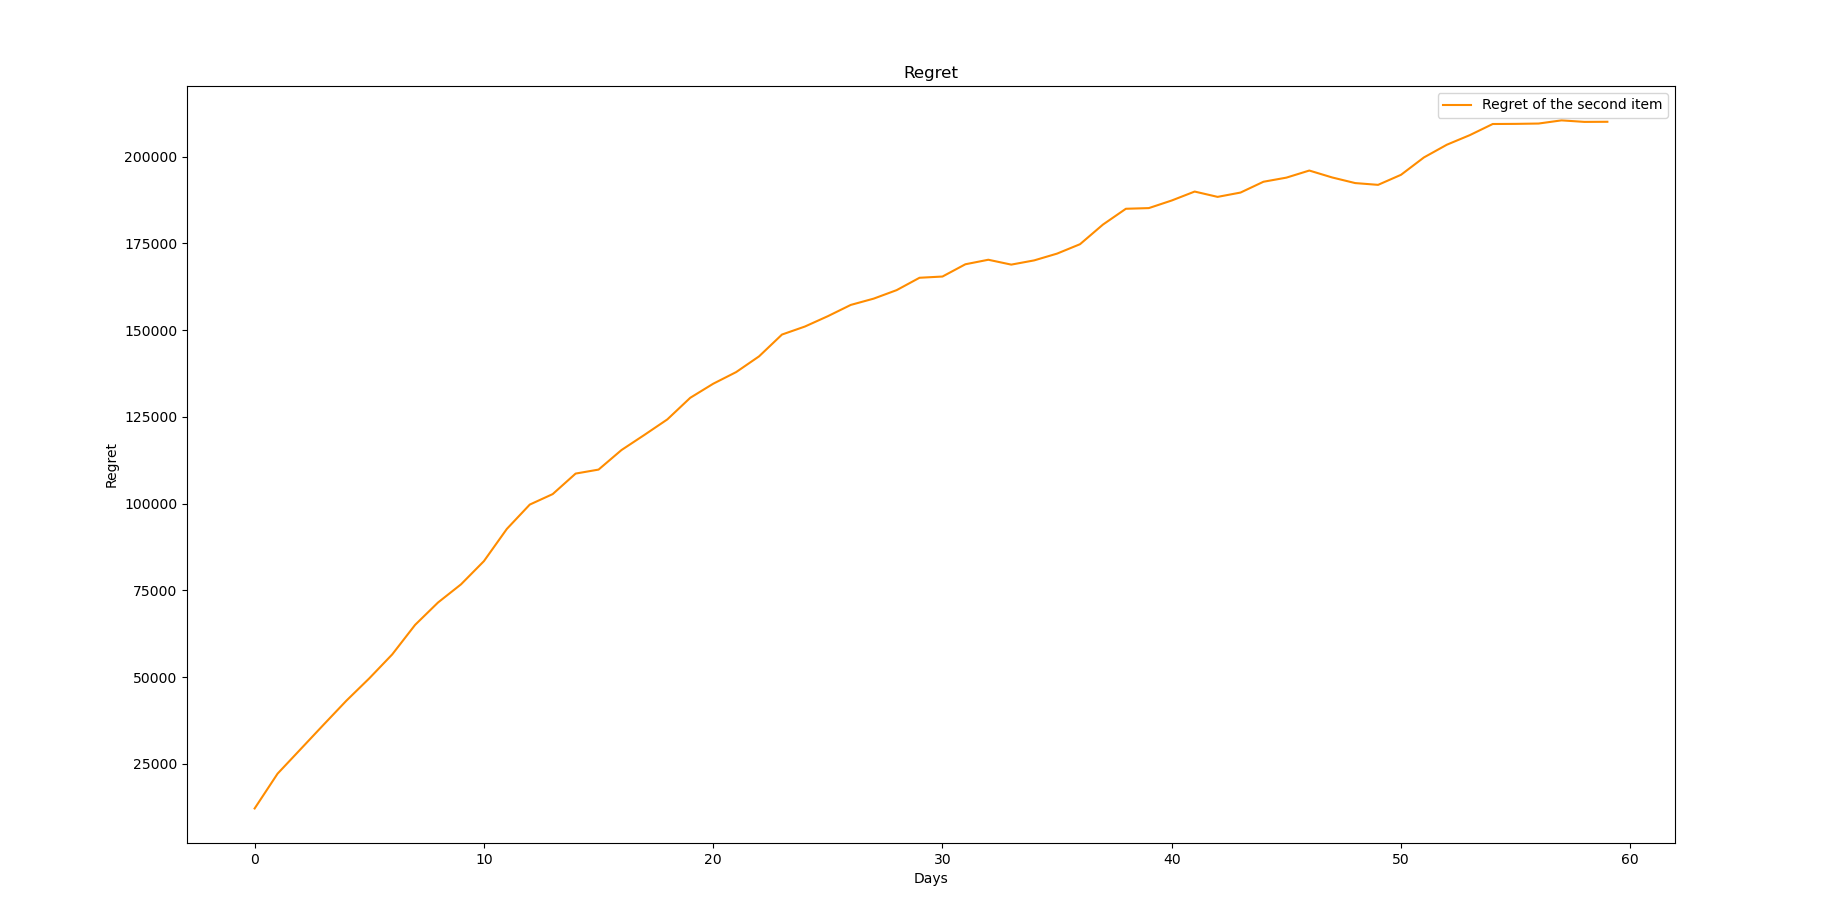
\includegraphics[scale=0.30]{Images/n5}
\end{center}
Days: 60\\
Experiments number: 5 \\
Starting delay of the Promo-Category UCB Matching: 1000 clients\\
UCB Matching at the end converge to the optimal solution \\
\subsection*{Considerations}
We can observe that the UCB Matching algorithm has a linear increase on the cumulative regret for the first thirty days, but after that, it becomes more and more stable on the optimal matching, and the cumulative regret does not increase so much.	
    %---
    \section*{Pricing and Matching problem}
    \label{sect:Pricing and Matching problem}
    \addcontentsline{toc}{section}{Pricing and Matching problem}
	\subparagraph*{Problem explaination}
\subparagraph*{Strategy}
\subparagraph*{Results}
\subparagraph*{Considerations}	
    %---
    \section*{Seasonal Pricing and Matching problem: Sliding Window}
    \label{sect:Seasonal Pricing and Matching problem: Sliding Window}
    \addcontentsline{toc}{section}{Seasonal Pricing and Matching problem: Sliding Window}
	\subparagraph*{Submission : }
\textit{Do the same as Step 6 when the conversion rates are not stationary. Adopt a sliding-window approach.}\\

The goal is the same of the previous problem, but in this case we are in a non-stationary environment, meaning that we have to introduce the seasonality. It is required to use a sliding-window approach.

Implementation: \textit{n7.py}
\subsection*{Basic knowledge}
\subparagraph*{Sliding Window Thompson Sampling (SWTS)} 
The Sliding Window Thompson Sampling is an alternative to the classical Thompson Sampling algorithm that is susceptible to changes. The main difference is the introduction of a parameter, the sliding window, of length $\tau\in \mathbb{N}$ such that the algorithm, at every round $t$, takes into account only the rewards obtained in the last $\tau$ rounds. Based on these realizations, we apply a TS-based algorithm to decide which is the arm to pull in the next round. In particular, the expected value of each arm is coupled with a posterior distribution from which we draw samples, and the arm with the highest value is the next arm to play.\\

\underline{\textit{Pseudocode}}\\
1. At every time $t$ for every arm $a$:

\hspace{2em}$\tilde{\theta_{a}} \leftarrow Sample(\mathbb P(\mu_{a}=\theta_{a}))$ \\

2. At every time $t$ play arm $a_{t}$ such that 

\hspace{2em}$a_{t} \leftarrow \argmax_{a \in A} \left\{ \tilde{\theta_{a}}  \right\} $ \\

3.  Update beta distribution of arm $a_{t}$

\hspace{2em}if $t\leq\tau$: $(\alpha_{a_{t}}, \beta_{a_{t}}) \leftarrow (\alpha_{a_{t}}, \beta_{a_{t}}) + (x_{a_{t},t}, 1 - x_{a_{t},t})$ 

\hspace{2em}if $\tau<t$:	$(\alpha_{a_{t}}, \beta_{a_{t}}) \leftarrow \max \left\{(1,1), (\alpha_{a_{t}}, \beta_{a_{t}}) + (x_{a_{t},t}, 1 - x_{a_{t},t}) - (x_{a_{t-\tau},t-\tau}, 1 - x_{a_{t-\tau},t-\tau})    \right\}$

\subsection*{Strategy}
The strategy is the same of the previous submission with the introduction of the seasonality. We use two learner that will retrieve the optimal superarm describing the couple of prices for the two items. One learner is the classical Thompson Sampling, the same used in the previous submission, while the other one is the Sliding Window Thompson Sampling. The size of the window used for the SWTS is computed as the $\sqrt{days * avgDailyCustomer} * \alpha$, where $days$ is the time horizon, $avgDailyCustomer = 1000$ is the normalizing factor used to compute the daily customer instances and $\alpha = 30 $ is a multiplicative factor empirically computed. Regarding the matching phase we do the same as the previous submission using a Promo-Category UCB learner for every superarm. In order to deal with seasonality, at the beginning of every new season all the matching learners are reset.

\subparagraph{Implementation} 
\begin{itemize}
	\item Conversion rates change according to the season
	\item The time horizon is equally divided into three seasons
	\item Candidates for the \textit{Racing Skis} are: \{2110.0, 1900.0, 2420.0, 2690.0\}
	\item Conversion rate associated with the first item is not known
	\item Candidates for the \textit{Racing Ski Helmet} are: \{360.0, 410.0, 530.0, 600.0\}
	\item Conversion rate associated with the second item is not known
	\item Optimal promotion-category assignment need to be learnt
\end{itemize}
\subparagraph{Optimal strategy}
The computation of the optimal strategy is the same performed in the previous submission but is calculated three times, taking into account the three seasons.
\begin{center}
	\begin{tabular}{|c|p{4cm}|p{4cm}|p{4cm}|} 
	\hline
	Season & \textit{Racing Skis optimal price} & \textit{Racing Ski Helmet} optimal price & Optimal promo-category matching \\ \hline
	\multirow{4}{*}{Spring-Summer} & \multirow{4}{*}{1900.0} & \multirow{4}{*}{410.0} & Sport addicted: P$_0$ = 0\% (410.0)  \\ 
								   & 					   &                      & Gifted: P$_2$ = 20\% (328.0)          \\ 
								   & 					   &                      & Worried: P$_3$ = 30\% (287.0)         \\
								   & 					   &                      & Amateur: P$_1$ = 10\% (369.0)         \\ \hline
	\multirow{4}{*}{Autumn} & \multirow{4}{*}{2690.0} & \multirow{4}{*}{530.0}  & Sport addicted: P$_1$ = 10\% (477.0)\\ 
								   & 					   &                      & Gifted: P$_3$ = 30\% (371.0)         \\ 
								   & 					   &                      & Worried: P$_2$ = 20\% (424.0)         \\
								   & 					   &                      & Amateur: P$_0$ = 0\% (530.0)         \\ \hline
	\multirow{4}{*}{Winter} & \multirow{4}{*}{2420.0} & \multirow{4}{*}{600.0}  & Sport addicted: P$_3$ = 30\% (420.0)\\ 
								   & 					   &                      & Gifted: P$_1$ = 10\% (540.0)         \\ 
								   & 					   &                      & Worried: P$_2$ = 20\% (480.0)         \\
								   & 					   &                      & Amateur: P$_0$ = 0\% (600.0)          \\ \hline
	\end{tabular}
\end{center}

\subsection*{Results}
\begin{center}
	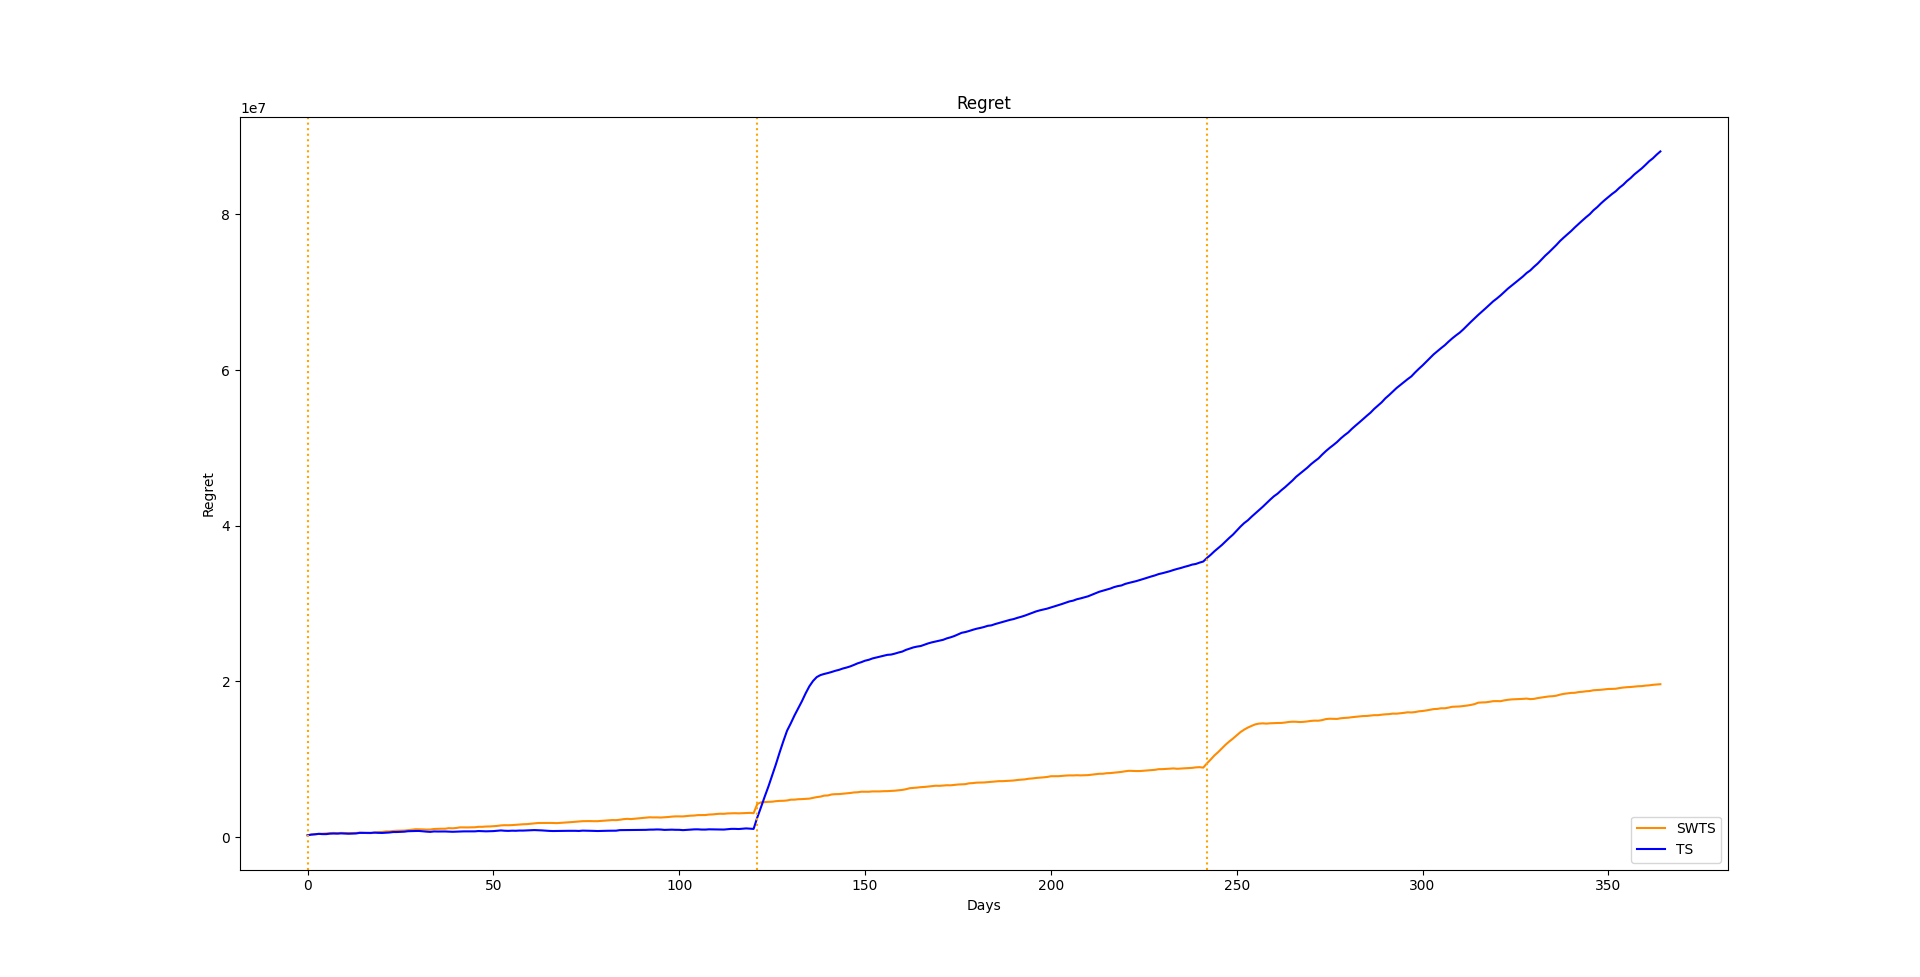
\includegraphics[scale=0.30]{Images/n7}
\end{center}
Days: 365\\
Number of seasons: 3 \\
Season length : $|365/3| = 122 $ days\\
Experiments number: 3 \\
Starting delay of the Promo-Category UCB Matching: 1000 clients\\
SWTS window size : $\sqrt{365 * 1000} * 30$\\
\subsection*{Considerations}
We can observe that in the first season the TS perform better since it has a complete knowledge of the collected samples, while the SWTS discards the older samples. However, when the conversion rates change, due to the change of the season, with the sliding window approach the newer samples become predominant. Thus, the algorithm changes its behaviour adapting the solution to the new season. We can note that the cumulative regret for the SWTS is about 4 times less than the TS. 	
    %---
    \section*{Seasonal Pricing and Matching problem: Change Detection}
    \label{sect:Seasonal Pricing and Matching problem: Change Detection}
    \addcontentsline{toc}{section}{Seasonal Pricing and Matching problem: Change Detection}
	\subparagraph*{Problem explaination}
\subparagraph*{Strategy}
\subparagraph*{Results}
\subparagraph*{Considerations}
     %---
     \section*{Folder Structure}
     \label{sect:Folder Structure}
     \addcontentsline{toc}{section}{Folder Structure}
     We have done a script file for every step of the project \textit{(n1.py, n3.py, n4.py, n5.py, n6.py, n7.py, n8.py)}. The first two steps are theoretical and they are included in this report, by the way we have implemented, for completeness, a script for the first step that find the optimal solution of the offline optimization problem.\\
In addition, we implemented the following codes, in order to compute the presented results. 
\subparagraph*{Config.py} is the configuration files and contains:
\begin{itemize}
	\item The samples used to reconstruct the demand curves of the two items
	\item The parameters of the customer distribution
	\item Other description information about the environment
\end{itemize} 

\subparagraph*{Context.py}
Context.py contains the definition of the class that simulates the behaviour of the context. All the experiments use this class. It is initialized with the values written in the config.py. It implements the methods related to the purchase of the two items based on their conversion rates, the generation of the daily customer numbers per class, the algorithm to calculate the optimal solutions for the non-stationary environment and the plot functions for the demand curves and the other distributions.


\subparagraph*{Algorithms folder}
The Algorithms folder contains all the learning algorithms: UCB and Thompson Sampling, with their customized version.

\subparagraph*{DIAnotebook.pdf}
It contains all the script files with the relative results.
    %---
    \label{sect:References}
    \addcontentsline{toc}{section}{References}
    \printbibliography[title={References}]
	%---	
\end{document}